% -*- root: ../../main.tex -*- %

\section{Design decisions} % (fold)
\label{sec:design_decisions}
  - GDVSEPC
  - wf engine partially in wf container
  - ruby / ruby on rails for readability and because i know it
    - drawback: speed, runtime

  - extra validator
    - defeats purpose of not sending data in gdvsepc but, just POC

  - for sake of simplicity:
    - no compiled language
% section design_decisions (end)

\section{Execution Images} % (fold)
\label{sec:execution_images}

  \subsection{Workflow Image} % (fold)
  \label{sub:workflow_container}
    - application
      - process instance
      - process definition
      - activity instance
      - file helper
      - configuration

  % subsection workflow_container (end)

  \subsection{Activity Image} % (fold)
  \label{sub:activity_containers}
    - application
      - configuration
      - file helper
  % subsection activity_containers (end)

% section execution_images (end)

\section{System Components} % (fold)
\label{sec:components_implementation}
  \subsection{Workflow Definition Service} % (fold)
    \label{sub:workflow_definition_service}
      - application
        - ruby on rails (api)
        - components
          - app logic
            - dockerhelper
            - image builder
            - image manager
          - controllers
          - models
            - activity
            - control-flow
            - process-definition
            - workflow
          - serializers
            - process definition image serializer
            - workflow full serializer

      - database
        - postgresql
      - data volume
        - docker volume

    \begin{figure}[htbp]
      \centering

      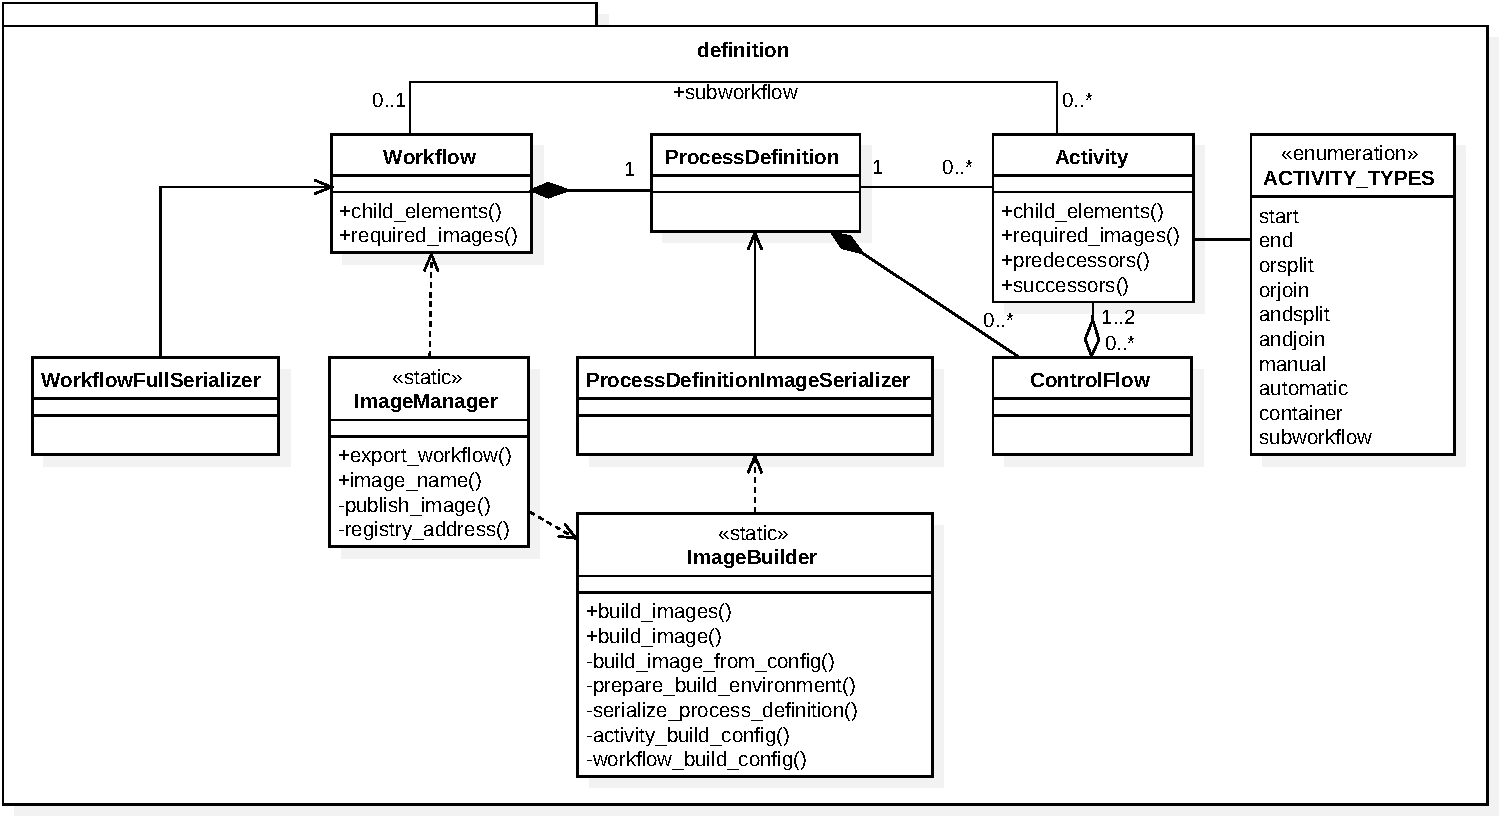
\includegraphics[width=0.95\textwidth]{content/images/class_diagram_definition-crop.pdf}
      \caption*{\scriptsize Controllers omitted for the sake of simplicity. Workflow, ProcessDefinition, Activity and ControlFlow each have a controller with the respective pluralized name plus a `Controller' suffix.}
      \caption{UML Class Diagram for the Definition Service}
      \label{fig:label}
    \end{figure}
    % subsection workflow_definition_service (end)

  \subsection{Organization Management Service} % (fold)
    \label{sub:organization_management_service}
      - application
        - controllers
        - models
          - role
            - ancestors
          - user
            - with role
      - database
        - postgresql
      - data volume
        - docker volume
    % subsection organization_management_service (end)

  \subsection{Worklist Service} % (fold)
    \label{sub:worklist_service}
      - application
        - controllers
        - models
          - worklist item
      - database
        - postgresql
      - data volume
        - docker volume
    % subsection worklist_service (end)

  \subsection{Workflow Engine Service} % (fold)
    \label{sub:workflow_engine_service}
      - application
    % subsection workflow_engine_service (end)

  \subsection{Developer Gateway} % (fold)
    \label{sub:developer_gateway}
      - application
        - backend: rails
        - frontend: angular app
    % subsection developer_gateway (end)

  \subsection{User Gateway} % (fold)
    \label{sub:user_gateway}
      - application
        - backend: rails
        - frontend: angular app
    % subsection user_gateway (end)

  \subsection{Message Oriented Middleware} % (fold)
    \label{sub:message_oriented_middleware}
      For this prototype, RabbitMQ was chosen as message oriented middleware, because it is well documented and has various ruby clients, \eg \emph{Hutch} and \emph{Bunny}.

      RabbitMQ exists as a pre-configured Docker image on the Docker Hub and can thus be utilized easily. The configuration of RabbitMQ in this image takes place when the respective container is run, which allows its configuration in the \texttt{docker-compose} configuration file.
      For the sake of simplicity, no authentication mechanism was introduced besides the simple default username/password combination.
    % subsection message_oriented_middleware (end)

  \subsection{Infrastructure Management Service} % (fold)
    \label{sub:infrastructure_management_service}
      - application
        - app logic
          - docker helper
          - environment manager
        - controllers
          - servers controller
        - models
          - server

    % subsection infrastructure_management_service (end)

  \subsection{Registry} % (fold)
    \label{sub:registry}
    % subsection registry (end)

  \subsection{Provisioning Service} % (fold)
    \label{sub:provisioning_service}
      - application
    % subsection provisioning_service (end)
% section components (end)


\begin{figure}[htbp]
  \centering
  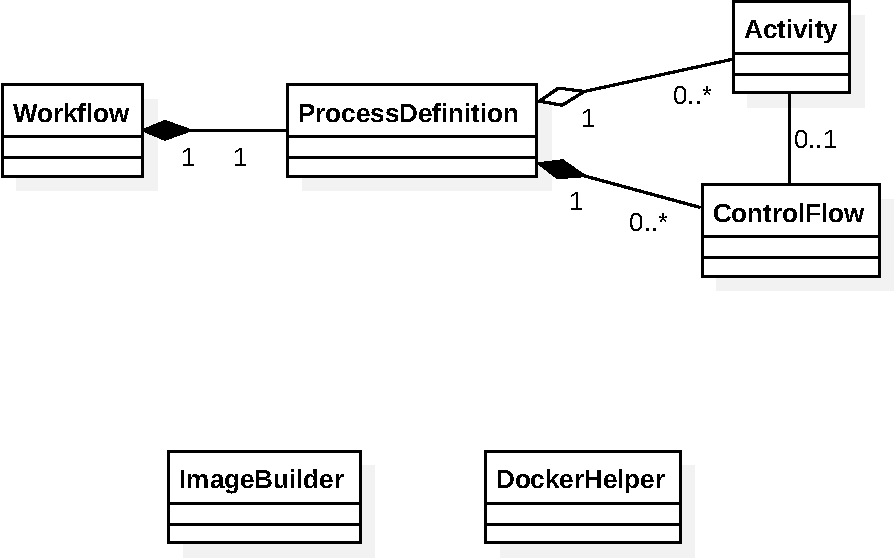
\includegraphics[width=0.95\textwidth]{content/images/class_d_definition-crop.pdf}
  \caption{UML Class Diagram for Workflowe Definition Service}
  \label{fig:uml_class_diagram_definition_service}
\end{figure}
